\documentclass[14pt]{extbook}
\usepackage{multicol, enumerate, enumitem, hyperref, color, soul, setspace, parskip, fancyhdr} %General Packages
\usepackage{amssymb, amsthm, amsmath, latexsym, units, mathtools} %Math Packages
\everymath{\displaystyle} %All math in Display Style
% Packages with additional options
\usepackage[headsep=0.5cm,headheight=12pt, left=1 in,right= 1 in,top= 1 in,bottom= 1 in]{geometry}
\usepackage[usenames,dvipsnames]{xcolor}
\usepackage{dashrule}  % Package to use the command below to create lines between items
\newcommand{\litem}[1]{\item#1\hspace*{-1cm}\rule{\textwidth}{0.4pt}}
\pagestyle{fancy}
\lhead{Progress Quiz 8}
\chead{}
\rhead{Version C}
\lfoot{5493-4176}
\cfoot{}
\rfoot{Summer C 2021}
\begin{document}

\begin{enumerate}
\litem{
Write the equation of the graph presented below in the form $f(x)=ax^2+bx+c$, assuming  $a=1$ or $a=-1$. Then, choose the intervals that $a, b,$ and $c$ belong to.
\begin{center}
    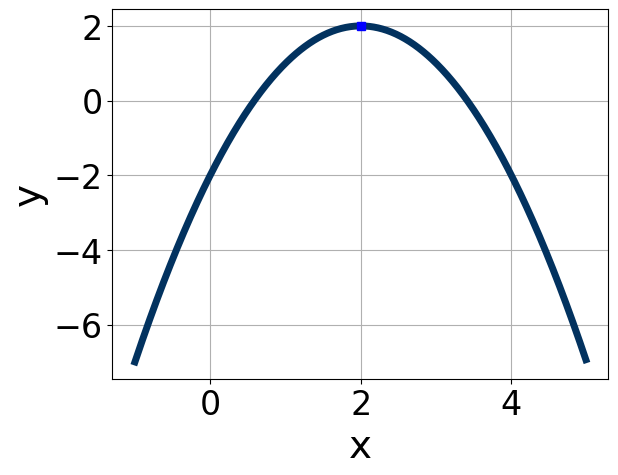
\includegraphics[width=0.5\textwidth]{../Figures/quadraticGraphToEquationC.png}
\end{center}
\begin{enumerate}[label=\Alph*.]
\item \( a \in [-1, 0], \hspace*{5mm} b \in [-6, -3], \text{ and } \hspace*{5mm} c \in [-4.1, -1.3] \)
\item \( a \in [-1, 0], \hspace*{5mm} b \in [3, 8], \text{ and } \hspace*{5mm} c \in [-4.1, -1.3] \)
\item \( a \in [-1, 0], \hspace*{5mm} b \in [-6, -3], \text{ and } \hspace*{5mm} c \in [-6.8, -4.6] \)
\item \( a \in [0, 3], \hspace*{5mm} b \in [3, 8], \text{ and } \hspace*{5mm} c \in [5.3, 6.8] \)
\item \( a \in [0, 3], \hspace*{5mm} b \in [-6, -3], \text{ and } \hspace*{5mm} c \in [5.3, 6.8] \)

\end{enumerate} }
\litem{
Factor the quadratic below. Then, choose the intervals that contain the constants in the form $(ax+b)(cx+d); b \leq d.$\[ 81x^{2} -27 x -10 \]\begin{enumerate}[label=\Alph*.]
\item \( a \in [26.84, 27.15], \hspace*{5mm} b \in [-8, -1], \hspace*{5mm} c \in [1.2, 3.4], \text{ and } \hspace*{5mm} d \in [1, 4] \)
\item \( a \in [8.76, 9.27], \hspace*{5mm} b \in [-8, -1], \hspace*{5mm} c \in [6.6, 13.6], \text{ and } \hspace*{5mm} d \in [1, 4] \)
\item \( a \in [0.38, 1.02], \hspace*{5mm} b \in [-48, -39], \hspace*{5mm} c \in [0.8, 1.4], \text{ and } \hspace*{5mm} d \in [18, 23] \)
\item \( a \in [1.84, 3.62], \hspace*{5mm} b \in [-8, -1], \hspace*{5mm} c \in [24.7, 28], \text{ and } \hspace*{5mm} d \in [1, 4] \)
\item \( \text{None of the above.} \)

\end{enumerate} }
\litem{
Solve the quadratic equation below. Then, choose the intervals that the solutions $x_1$ and $x_2$ belong to, with $x_1 \leq x_2$.\[ 10x^{2} +33 x -54 = 0 \]\begin{enumerate}[label=\Alph*.]
\item \( x_1 \in [-13.5, -12.5] \text{ and } x_2 \in [0.11, 0.52] \)
\item \( x_1 \in [-6.5, -3.5] \text{ and } x_2 \in [1.14, 1.33] \)
\item \( x_1 \in [-1.5, 4.5] \text{ and } x_2 \in [3.34, 3.77] \)
\item \( x_1 \in [-13, -8] \text{ and } x_2 \in [0.49, 0.76] \)
\item \( x_1 \in [-46, -44] \text{ and } x_2 \in [11.7, 12.23] \)

\end{enumerate} }
\litem{
Write the equation of the graph presented below in the form $f(x)=ax^2+bx+c$, assuming  $a=1$ or $a=-1$. Then, choose the intervals that $a, b,$ and $c$ belong to.
\begin{center}
    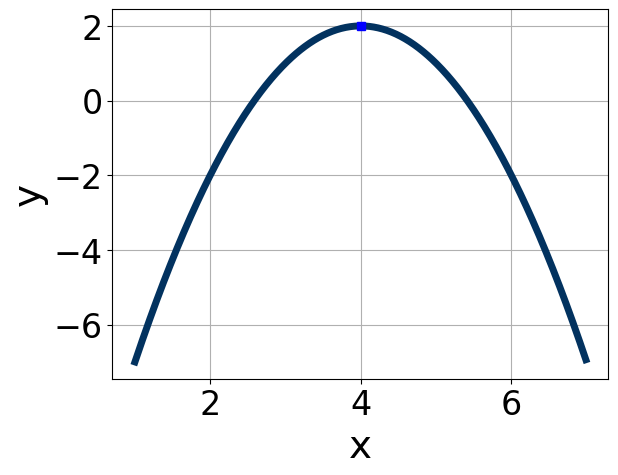
\includegraphics[width=0.5\textwidth]{../Figures/quadraticGraphToEquationCopyC.png}
\end{center}
\begin{enumerate}[label=\Alph*.]
\item \( a \in [0, 5], \hspace*{5mm} b \in [-11, -7], \text{ and } \hspace*{5mm} c \in [17, 20] \)
\item \( a \in [-6, 0], \hspace*{5mm} b \in [8, 10], \text{ and } \hspace*{5mm} c \in [-14, -12] \)
\item \( a \in [-6, 0], \hspace*{5mm} b \in [-11, -7], \text{ and } \hspace*{5mm} c \in [-18, -16] \)
\item \( a \in [0, 5], \hspace*{5mm} b \in [8, 10], \text{ and } \hspace*{5mm} c \in [17, 20] \)
\item \( a \in [-6, 0], \hspace*{5mm} b \in [-11, -7], \text{ and } \hspace*{5mm} c \in [-14, -12] \)

\end{enumerate} }
\litem{
Solve the quadratic equation below. Then, choose the intervals that the solutions belong to, with $x_1 \leq x_2$ (if they exist).\[ -20x^{2} -13 x + 3 = 0 \]\begin{enumerate}[label=\Alph*.]
\item \( x_1 \in [-1.46, -0.41] \text{ and } x_2 \in [-0.43, 0.72] \)
\item \( x_1 \in [-4.25, -3.01] \text{ and } x_2 \in [15.81, 16.8] \)
\item \( x_1 \in [-21.08, -20.1] \text{ and } x_2 \in [18.98, 20.41] \)
\item \( x_1 \in [-0.59, -0.06] \text{ and } x_2 \in [0.27, 1.63] \)
\item \( \text{There are no Real solutions.} \)

\end{enumerate} }
\litem{
Factor the quadratic below. Then, choose the intervals that contain the constants in the form $(ax+b)(cx+d); b \leq d.$\[ 36x^{2} -60 x + 25 \]\begin{enumerate}[label=\Alph*.]
\item \( a \in [4.75, 6.2], \hspace*{5mm} b \in [-8, -4], \hspace*{5mm} c \in [5.94, 6.09], \text{ and } \hspace*{5mm} d \in [-7, -3] \)
\item \( a \in [0.76, 1.49], \hspace*{5mm} b \in [-34, -25], \hspace*{5mm} c \in [0.54, 1.72], \text{ and } \hspace*{5mm} d \in [-33, -26] \)
\item \( a \in [1.42, 2.16], \hspace*{5mm} b \in [-8, -4], \hspace*{5mm} c \in [17.56, 18.04], \text{ and } \hspace*{5mm} d \in [-7, -3] \)
\item \( a \in [17.82, 18.42], \hspace*{5mm} b \in [-8, -4], \hspace*{5mm} c \in [1.88, 2.43], \text{ and } \hspace*{5mm} d \in [-7, -3] \)
\item \( \text{None of the above.} \)

\end{enumerate} }
\litem{
Graph the equation below.\[ f(x) = -(x-2)^2 + 18 \]\begin{enumerate}[label=\Alph*.]
\begin{multicols}{2}\item 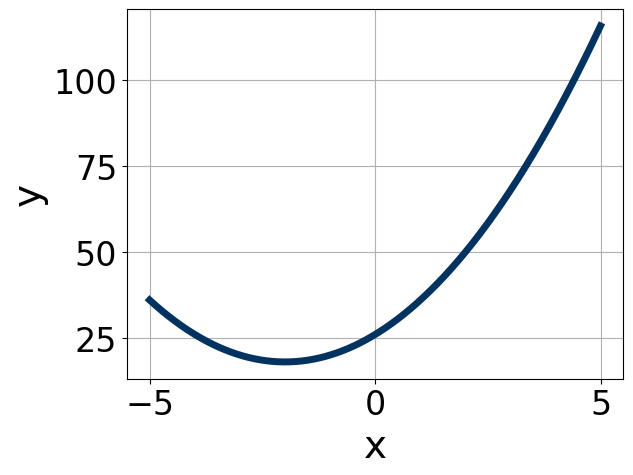
\includegraphics[width = 0.3\textwidth]{../Figures/quadraticEquationToGraphAC.png}\item 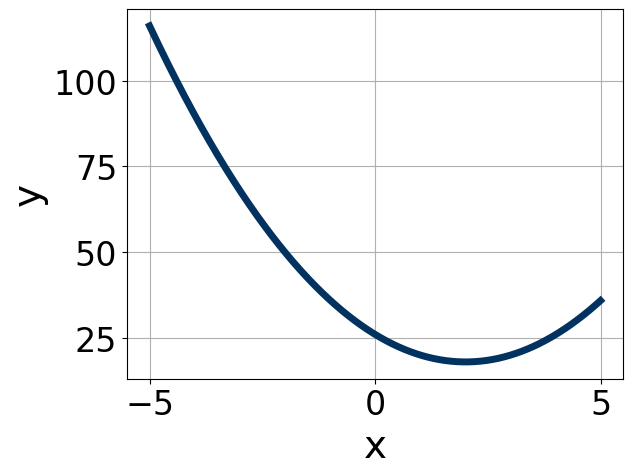
\includegraphics[width = 0.3\textwidth]{../Figures/quadraticEquationToGraphBC.png}\item 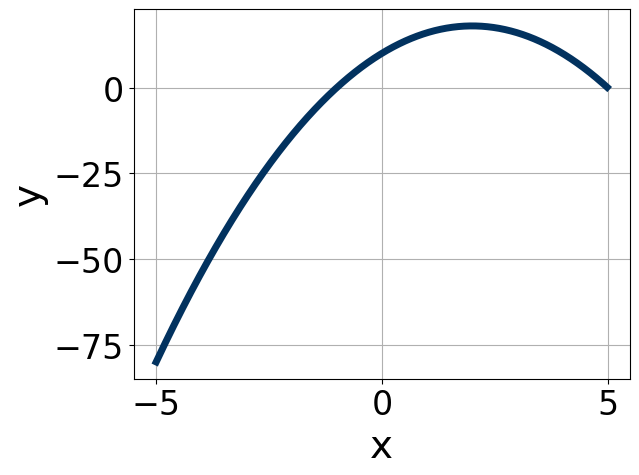
\includegraphics[width = 0.3\textwidth]{../Figures/quadraticEquationToGraphCC.png}\item 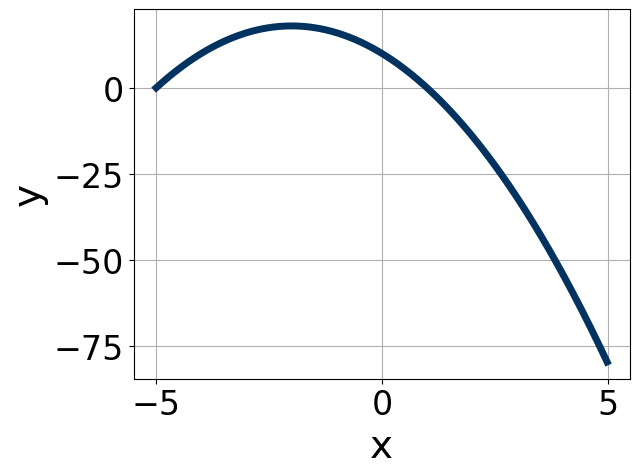
\includegraphics[width = 0.3\textwidth]{../Figures/quadraticEquationToGraphDC.png}\end{multicols}\item None of the above.
\end{enumerate} }
\litem{
Solve the quadratic equation below. Then, choose the intervals that the solutions belong to, with $x_1 \leq x_2$ (if they exist).\[ 15x^{2} +8 x -5 = 0 \]\begin{enumerate}[label=\Alph*.]
\item \( x_1 \in [-1.09, -0.48] \text{ and } x_2 \in [0.05, 0.52] \)
\item \( x_1 \in [-0.82, -0.3] \text{ and } x_2 \in [0.86, 1.21] \)
\item \( x_1 \in [-20.11, -18.33] \text{ and } x_2 \in [18.23, 19.14] \)
\item \( x_1 \in [-14.16, -13.12] \text{ and } x_2 \in [5.25, 5.92] \)
\item \( \text{There are no Real solutions.} \)

\end{enumerate} }
\litem{
Solve the quadratic equation below. Then, choose the intervals that the solutions $x_1$ and $x_2$ belong to, with $x_1 \leq x_2$.\[ 10x^{2} +57 x + 54 = 0 \]\begin{enumerate}[label=\Alph*.]
\item \( x_1 \in [-9.26, -8.66] \text{ and } x_2 \in [-0.62, -0.53] \)
\item \( x_1 \in [-4.2, -3.05] \text{ and } x_2 \in [-1.52, -1.39] \)
\item \( x_1 \in [-14.3, -13.15] \text{ and } x_2 \in [-0.49, -0.39] \)
\item \( x_1 \in [-4.83, -3.98] \text{ and } x_2 \in [-1.44, -1.11] \)
\item \( x_1 \in [-45.02, -44.91] \text{ and } x_2 \in [-12.01, -11.94] \)

\end{enumerate} }
\litem{
Graph the equation below.\[ f(x) = -(x+4)^2 + 16 \]\begin{enumerate}[label=\Alph*.]
\begin{multicols}{2}\item 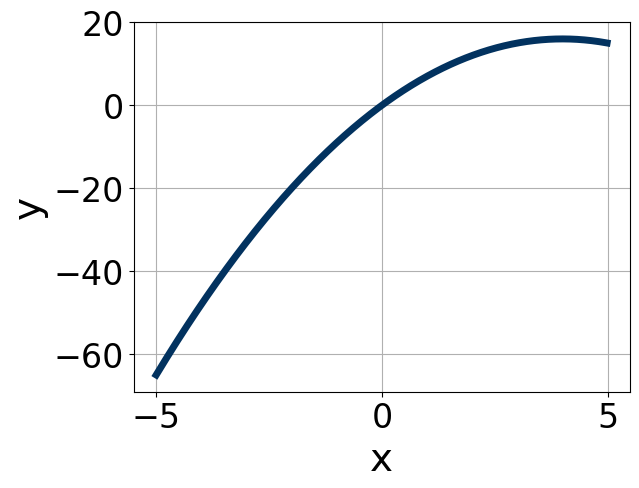
\includegraphics[width = 0.3\textwidth]{../Figures/quadraticEquationToGraphCopyAC.png}\item 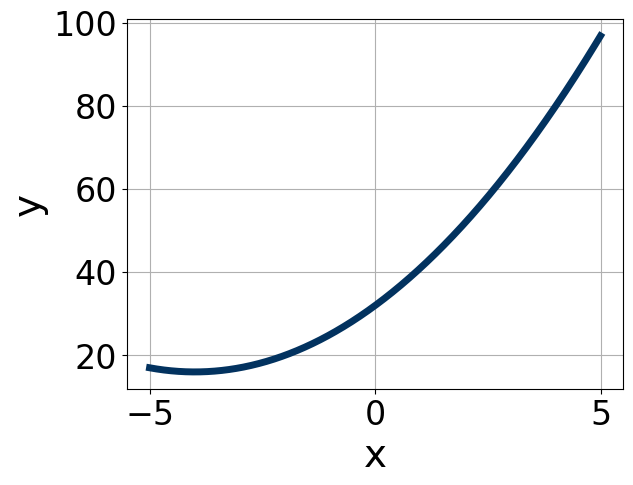
\includegraphics[width = 0.3\textwidth]{../Figures/quadraticEquationToGraphCopyBC.png}\item 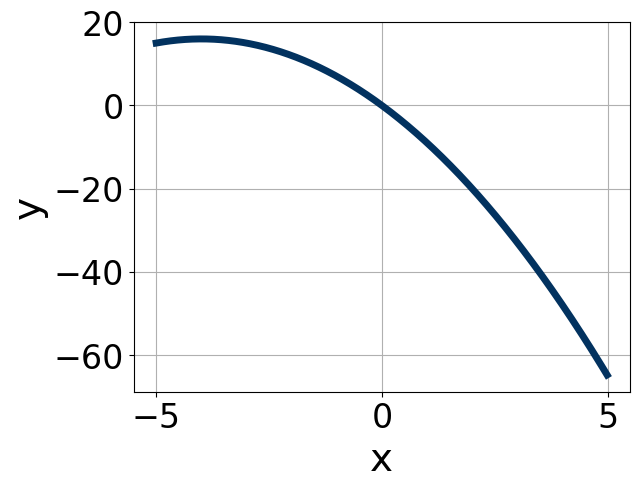
\includegraphics[width = 0.3\textwidth]{../Figures/quadraticEquationToGraphCopyCC.png}\item 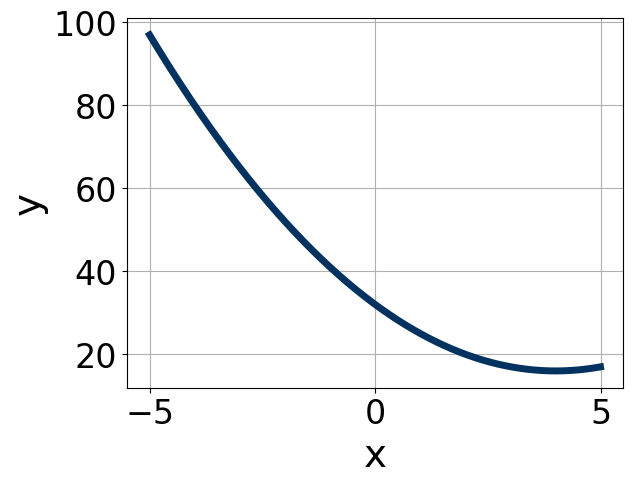
\includegraphics[width = 0.3\textwidth]{../Figures/quadraticEquationToGraphCopyDC.png}\end{multicols}\item None of the above.
\end{enumerate} }
\end{enumerate}

\end{document}